
\documentclass[10pt,twocolumn]{article}

\usepackage[utf8]{inputenc}
\usepackage[T1]{fontenc}
\usepackage[portuguese]{babel}
\usepackage[a4paper,margin=1.9cm,columnsep=0.7cm]{geometry}
\usepackage{graphicx}
\usepackage{booktabs}
\usepackage{array}
\usepackage{caption}
\usepackage{xcolor}
\usepackage{tcolorbox}
\usepackage{fancyhdr}
\usepackage[hidelinks]{hyperref}
\usepackage{titlesec}
\usepackage{enumitem}
\usepackage{float}
\usepackage{amsmath}
\usepackage{url}

\definecolor{estgblue}{HTML}{1F5C99}

\titleformat{\section}{\large\bfseries\color{estgblue}}{\thesection.}{0.5em}{}
\titleformat{\subsection}{\bfseries}{\thesubsection}{0.5em}{}

\pagestyle{fancy}
\fancyhf{}
\renewcommand{\headrulewidth}{0.4pt}
\fancyhead[R]{\small\itshape Deteção de Fraude e Risco Financeiro com Regressão Logística, Decision Tree e Random Forest}
\fancyfoot[C]{\small\thepage}

\setlength{\parskip}{0.4em}
\setlength{\parindent}{0pt}
\captionsetup{font=small,labelfont=bf}

\newcommand{\authorline}{Nelson Araújo \; -- \; N.\textordmasculine{} de aluno: 20743\\Ivo Pimenta \; -- \; N.\textordmasculine{} de aluno: a37326}
\newcommand{\logoimg}{
\includegraphics[width=3.2cm]{../figuresextra/logo.png}}

\newtcolorbox{resumobox}{colframe=estgblue,colback=estgblue!5,boxrule=0.6pt,left=6pt,right=6pt,top=4pt,bottom=4pt,arc=2pt}

\begin{document}

\twocolumn[
  \begin{center}
    \logoimg\\
    \vspace{0.4em}
    {\bfseries Escola Superior de Tecnologia -- Instituto Politécnico do Cávado e do Ave (IPCA)}\\
    {\small Pós-Graduação em Cibersegurança e Informática Forense (2025/2026)}\\
    {\small Unidade Curricular: Inteligência Artificial para Cibersegurança}\\
    \vspace{0.8em}
    {\Large\bfseries Deteção de Fraude e Risco Financeiro com Regressão Logística, Decision Tree e Random Forest}\\
    \vspace{0.3em}
    {\itshape Comparação de Três Classificadores Supervisionados em Dois Conjuntos de Dados: Bank Marketing e Credit Card Fraud}\\
    \vspace{0.6em}
    \authorline\\
    {\small Barcelos, Portugal, 2026}\\
    \vspace{0.8em}
  \end{center}

  \begin{resumobox}
    {\bfseries\color{estgblue} Resumo -- } \textit{Este artigo apresenta uma abordagem simples e reprodutível para classificação supervisionada em contexto financeiro, com foco na deteção de risco operacional e fraude. Foram utilizados dois conjuntos de dados de natureza distinta: o \textit{Bank Marketing}, associado à previsão de adesão a depósitos bancários, e o \textit{Credit Card Fraud}, associado à identificação de transações fraudulentas. A escolha destes datasets permite avaliar o comportamento dos modelos em dois cenários diferentes: um problema financeiro quase balanceado, com variáveis categóricas e numéricas, e um problema fortemente desbalanceado, típico da deteção de fraude. Foram comparados três classificadores supervisionados clássicos: Regressão Logística, Decision Tree e Random Forest. A avaliação recorreu às métricas accuracy, precision, recall, F1-score, ROC-AUC e Average Precision, complementadas por análise exploratória, distribuição dos casos, matrizes de confusão, curvas ROC, curvas Precision-Recall e comparação gráfica do F1-score. Os resultados mostram que o Random Forest obteve o melhor F1-score nos dois datasets, alcançando 0,8403 no Bank Marketing e 0,9170 no Credit Card Fraud. No dataset de fraude, a Regressão Logística obteve o recall mais elevado, mas com precision inferior, revelando maior tendência para gerar falsos positivos. A análise confirma que, em problemas de cibersegurança financeira, a accuracy isolada é insuficiente, sendo necessário considerar métricas sensíveis ao desequilíbrio entre classes.}

    \textbf{Palavras-chave:} fraude financeira, machine learning supervisionado, Regressão Logística, Decision Tree, Random Forest, classificação binária, cibersegurança, datasets desbalanceados.
  \end{resumobox}
  \vspace{0.6em}
]

\section{Introdução}
A digitalização dos serviços financeiros aumentou a rapidez e a disponibilidade de pagamentos, transferências e operações bancárias, mas também ampliou a superfície de ataque disponível para fraude, abuso e utilização indevida de sistemas. Em ambientes de banca online e pagamentos eletrónicos, uma única transação fraudulenta pode representar perda financeira, exposição de dados pessoais, quebra de confiança e necessidade de intervenção humana posterior. Por este motivo, a deteção automática de padrões suspeitos é um problema relevante de cibersegurança aplicada.

A aprendizagem supervisionada é adequada para este tipo de problema quando existem exemplos históricos rotulados. A partir de registos classificados como legítimos ou suspeitos, os modelos conseguem aprender relações entre os atributos das operações e a classe final. O objetivo não é substituir completamente a análise humana, mas sim apoiar a triagem, priorizar alertas e reduzir o tempo necessário para identificar situações de risco.

Este trabalho compara três algoritmos supervisionados em dois datasets financeiros. A pergunta de investigação central é: qual dos modelos -- Regressão Logística, Decision Tree ou Random Forest -- apresenta melhor desempenho em cenários financeiros com características e níveis de desequilíbrio diferentes? Para responder a esta questão, a mesma metodologia experimental foi aplicada ao dataset Bank Marketing e ao dataset Credit Card Fraud, usando divisão treino/teste estratificada e as mesmas métricas de avaliação.

A escolha dos três modelos permite uma comparação direta entre abordagens com propriedades distintas. A Regressão Logística representa uma modelo de referência linear, simples e interpretável. A Decision Tree oferece uma estrutura de decisão intuitiva e capaz de modelar relações não lineares, mas pode ser sensível a variações nos dados. O Random Forest combina várias árvores de decisão, reduzindo a variância e aumentando a robustez, embora com menor interpretabilidade direta.

\section{Trabalhos Relacionados}
A deteção de fraude com aprendizagem automática tem sido estudada em diferentes contextos financeiros, incluindo cartões de crédito, transações bancárias e sistemas de pagamento. Dal Pozzolo et al. analisaram lições práticas da deteção de fraude em cartões de crédito, destacando a dificuldade causada pelo forte desequilíbrio entre transações legítimas e fraudulentas \cite{dalpozzolo2014credit}. Este aspeto é essencial, porque num dataset real de fraude a classe positiva tende a representar apenas uma fração muito pequena dos registos.

Moro, Cortez e Rita estudaram o uso de técnicas de \textit{data mining} em campanhas de marketing bancário, mostrando que modelos supervisionados podem apoiar decisões em contexto financeiro e comercial \cite{moro2014data}. Embora o objetivo do Bank Marketing não seja fraude no sentido estrito, o dataset é útil neste trabalho por representar um problema financeiro de classificação binária com variáveis reais, categóricas e numéricas.

A Regressão Logística é frequentemente usada como modelo de referência em problemas de classificação por ser eficiente, robusta e relativamente interpretável. As árvores de decisão são úteis pela interpretabilidade das regras aprendidas, mas podem sofrer de sobreajuste quando usadas isoladamente. O Random Forest, proposto por Breiman, reduz este problema através da combinação de múltiplas árvores treinadas sobre subconjuntos diferentes dos dados \cite{breiman2001random}. Do ponto de vista de implementação, bibliotecas como o scikit-learn permitem construir fluxos de processamento reprodutíveis, integrando pré-processamento, treino e avaliação dos modelos \cite{pedregosa2011scikit}.

\section{Modelo de IA/ML}
\subsection{Datasets}
Foram utilizados dois datasets públicos fornecidos no projeto, ambos tratados como problemas de classificação binária. A Tabela~\ref{tab:datasets} apresenta o número de registos, número de atributos, distribuição dos casos e taxa da classe positiva.

\begin{table}[H]
\centering
\caption{Resumo dos datasets utilizados.}
\label{tab:datasets}
\resizebox{\linewidth}{!}{%
\begin{tabular}{lrrrrr}
\toprule
Dataset & Registos & Atrib. & Negativos & Positivos & Pos. \\
\midrule
Credit Card Fraud & 15492 & 30 & 15000 & 492 & 3,18\% \\
Bank Marketing & 11162 & 16 & 5873 & 5289 & 47,38\% \\
\bottomrule
\end{tabular}%
}
\end{table}

Na Tabela~\ref{tab:datasets}, a coluna \textit{Negativos} representa os casos normais ou de não adesão, dependendo do dataset. A coluna \textit{Positivos} representa os casos de interesse: no Bank Marketing corresponde aos clientes que aderiram ao depósito; no Credit Card Fraud corresponde às transações fraudulentas. Esta designação torna a leitura mais clara do que usar apenas os rótulos numéricos 0 e 1.

O dataset Bank Marketing contém registos associados a campanhas bancárias. A variável alvo é \texttt{deposit}, convertida para classificação binária, em que o caso positivo representa a resposta \texttt{yes}, ou seja, o cliente aderiu ao depósito. Apesar de não corresponder diretamente a fraude, este dataset pertence ao domínio financeiro e permite avaliar classificação operacional num cenário relativamente equilibrado.

O dataset Credit Card Fraud contém transações de cartão de crédito, onde a variável alvo é \texttt{Class}: valor 1 para fraude e 0 para transação normal. Este dataset é muito mais desbalanceado, com apenas 3,18\% de exemplos positivos na versão usada no projeto. Esta característica aproxima o problema de cenários reais de cibersegurança, em que os eventos maliciosos são raros face ao volume total de atividade legítima.

\begin{figure}[H]
\centering
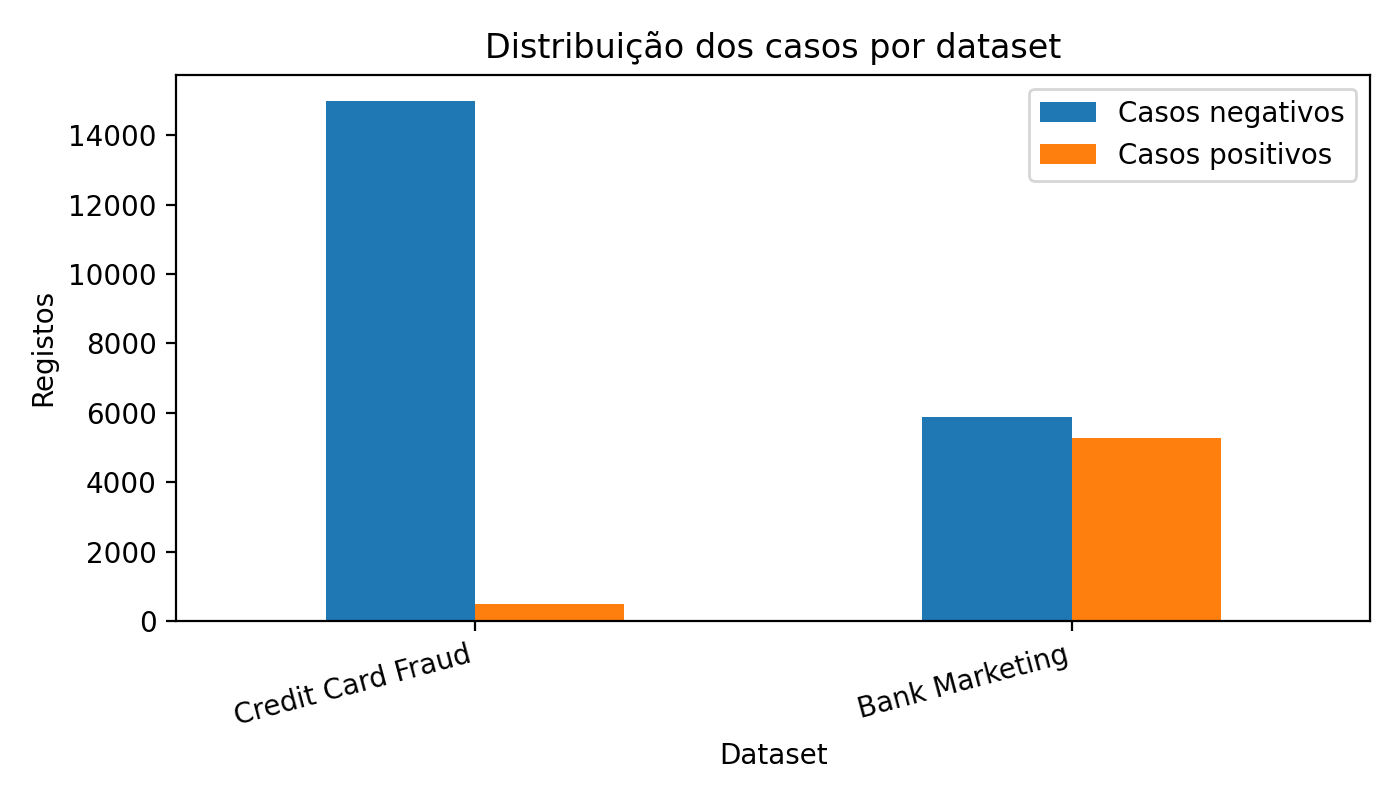
\includegraphics[width=0.95\linewidth]{../figures/class_distribution.png}
\caption{Distribuição dos casos nos dois datasets.}
\label{fig:classdist}
\end{figure}

A Figura~\ref{fig:classdist} confirma a diferença entre os datasets. No Bank Marketing, as classes estão relativamente próximas, pelo que a accuracy pode refletir melhor o desempenho global. No Credit Card Fraud, a accuracy pode ser enganadora: um modelo que classificasse quase tudo como legítimo teria accuracy elevada, mas falharia o objetivo de detetar fraude. Por isso, F1-score, recall, precision, ROC-AUC e Average Precision são métricas essenciais.

\subsection{Análise exploratória inicial}
Antes do treino foi realizada uma análise exploratória simples no notebook. Esta etapa consistiu em carregar os datasets, visualizar as primeiras linhas com \texttt{head()}, verificar a distribuição da variável alvo e confirmar a dimensão dos dados. Esta inspeção é importante porque permite garantir que os ficheiros foram carregados corretamente, que a variável alvo foi identificada e que a estrutura dos atributos é compatível com o fluxo de processamento de treino.

No Credit Card Fraud, os atributos são essencialmente numéricos, incluindo variáveis transformadas e o valor da transação. No Bank Marketing, existem atributos numéricos e categóricos, como idade, profissão, estado civil, educação, saldo, contacto e histórico de campanha. Esta diferença justifica a necessidade de pré-processamento adequado antes do treino dos modelos.

\subsection{Pré-processamento}
O fluxo de processamento experimental foi desenhado para ser simples, reproduzível e aplicável aos dois datasets. No Bank Marketing, as variáveis categóricas foram codificadas através de \textit{One-Hot Encoding}, enquanto as variáveis numéricas foram tratadas de forma compatível com os classificadores usados. No Credit Card Fraud, os atributos numéricos foram usados diretamente após a preparação necessária.

Em ambos os casos foi aplicada divisão treino/teste estratificada, preservando a proporção das classes nos conjuntos de treino e teste. Esta decisão é particularmente importante para o dataset de fraude, uma vez que uma divisão aleatória não estratificada poderia produzir conjuntos de teste com poucos exemplos positivos e tornar a avaliação instável. O mesmo split foi usado para comparar os três modelos dentro de cada dataset, garantindo uma comparação justa.

\subsection{Modelos}
Foram usados apenas três modelos supervisionados. O primeiro é a Regressão Logística, um classificador linear adequado como modelo de referência, sobretudo quando se pretende uma solução simples, rápida e interpretável. Este modelo estima a probabilidade de pertença à classe positiva e permite analisar diretamente o compromisso entre falsos positivos e falsos negativos através do limiar de decisão.

O segundo modelo é a Decision Tree. Este classificador divide o espaço de atributos através de regras sucessivas, o que facilita a interpretação do processo de decisão. Contudo, uma árvore única pode ajustar-se demasiado ao conjunto de treino, especialmente quando existem padrões ruidosos ou variáveis com interações complexas.

O terceiro modelo é o Random Forest, um ensemble de árvores de decisão. Ao combinar várias árvores, o modelo tende a ser mais robusto do que uma Decision Tree isolada, reduzindo a variância e melhorando a capacidade de generalização. Em contrapartida, o custo computacional e a dificuldade de interpretação aumentam.

\subsection{Estrutura do código}
O projeto encontra-se organizado com separação entre dados, código, figuras, referências e relatórios. O código principal está no ficheiro \texttt{src/fraud\_modeling.py}, que implementa o carregamento dos datasets, o pré-processamento, a divisão treino/teste, o treino dos três modelos e a geração das métricas. O notebook de apresentação reproduz o fluxo experimental de forma visual e comentada, permitindo mostrar a análise feita aos datasets, os modelos escolhidos e os resultados obtidos.

\section{Resultados e Discussão}
\subsection{Protocolo experimental e métricas}
Os três modelos foram avaliados nos dois datasets com as mesmas métricas: accuracy, precision, recall, F1-score, ROC-AUC e Average Precision. A Tabela~\ref{tab:metricas} resume o significado de cada métrica usada.

\begin{table}[H]
\centering
\caption{Significado das métricas utilizadas.}
\label{tab:metricas}
\scriptsize
\begin{tabular}{p{0.28\linewidth}p{0.62\linewidth}}
\toprule
Métrica & Significado \\
\midrule
Accuracy & Percentagem total de classificações corretas. \\
Precision & Das previsões positivas, quantas eram realmente positivas. \\
Recall & Dos casos positivos reais, quantos foram detetados. \\
F1-score & Equilíbrio entre precision e recall. \\
ROC-AUC & Capacidade geral de separar as duas classes. \\
Average Precision & Métrica útil em datasets desbalanceados, baseada na curva Precision-Recall. \\
\bottomrule
\end{tabular}
\end{table}

Para problemas de fraude, a análise privilegia o F1-score, o recall e a Average Precision, porque estas métricas são mais informativas em cenários desbalanceados. A precision indica a proporção de alertas positivos que são realmente positivos, enquanto o recall indica a proporção de casos positivos que o modelo conseguiu detetar. O F1-score foi usado como métrica principal porque combina estes dois aspetos.

\subsection{Resultados no Bank Marketing}
A Tabela~\ref{tab:bank} apresenta os resultados no dataset Bank Marketing. O Random Forest obteve o melhor F1-score (0,8403), seguido da Regressão Logística (0,8251) e da Decision Tree (0,8196). A diferença entre Regressão Logística e Decision Tree é reduzida, mas o Random Forest apresentou melhor equilíbrio entre precision e recall.

\begin{table}[H]
\centering
\caption{Métricas de desempenho no Bank Marketing.}
\label{tab:bank}
\resizebox{\linewidth}{!}{%
\begin{tabular}{lrrrrrr}
\toprule
Modelo & Acc. & Prec. & Rec. & F1 & ROC & AP \\
\midrule
Random Forest & 0,8402 & 0,7980 & 0,8873 & 0,8403 & 0,9132 & 0,8841 \\
Reg. Logística & 0,8341 & 0,8242 & 0,8260 & 0,8251 & 0,9096 & 0,8700 \\
Decision Tree & 0,8255 & 0,8032 & 0,8366 & 0,8196 & 0,8668 & 0,8142 \\
\bottomrule
\end{tabular}%
}
\end{table}

Neste dataset, as classes estão relativamente equilibradas, o que ajuda a obter métricas mais próximas entre si. A Regressão Logística apresenta precision ligeiramente superior à Decision Tree, mas recall inferior. O Random Forest consegue aumentar o recall mantendo uma precision competitiva, explicando o melhor F1-score.

\subsection{Resultados no Credit Card Fraud}
A Tabela~\ref{tab:credit} apresenta os resultados no dataset Credit Card Fraud. O Random Forest voltou a obter o melhor F1-score (0,9170), com precision elevada (0,9906) e recall de 0,8537. A Regressão Logística obteve o recall mais elevado (0,9024), mas a sua precision foi bastante inferior (0,5812), indicando maior número de falsos positivos. A Decision Tree ficou numa posição intermédia.

\begin{table}[H]
\centering
\caption{Métricas de desempenho no Credit Card Fraud.}
\label{tab:credit}
\resizebox{\linewidth}{!}{%
\begin{tabular}{lrrrrrr}
\toprule
Modelo & Acc. & Prec. & Rec. & F1 & ROC & AP \\
\midrule
Random Forest & 0,9951 & 0,9906 & 0,8537 & 0,9170 & 0,9777 & 0,9199 \\
Decision Tree & 0,9863 & 0,7778 & 0,7967 & 0,7871 & 0,8964 & 0,7194 \\
Reg. Logística & 0,9762 & 0,5812 & 0,9024 & 0,7070 & 0,9882 & 0,9233 \\
\bottomrule
\end{tabular}%
}
\end{table}

A accuracy é muito elevada em todos os modelos, mas neste dataset deve ser interpretada com cuidado. Como a classe fraude é rara, a accuracy pode ocultar erros relevantes na classe positiva. Por exemplo, a Regressão Logística tem accuracy de 0,9762, mas F1-score de apenas 0,7070, devido à baixa precision. Isto demonstra que a accuracy isolada não é suficiente para avaliar um detetor de fraude.

\subsection{Matrizes de confusão}
A matriz de confusão permite observar os acertos e os erros do modelo. Os verdadeiros negativos correspondem a casos normais classificados como normais; os verdadeiros positivos correspondem a casos positivos corretamente detetados; os falsos positivos são casos normais sinalizados como positivos; e os falsos negativos são casos positivos que não foram detetados.

\begin{figure}[H]
\centering
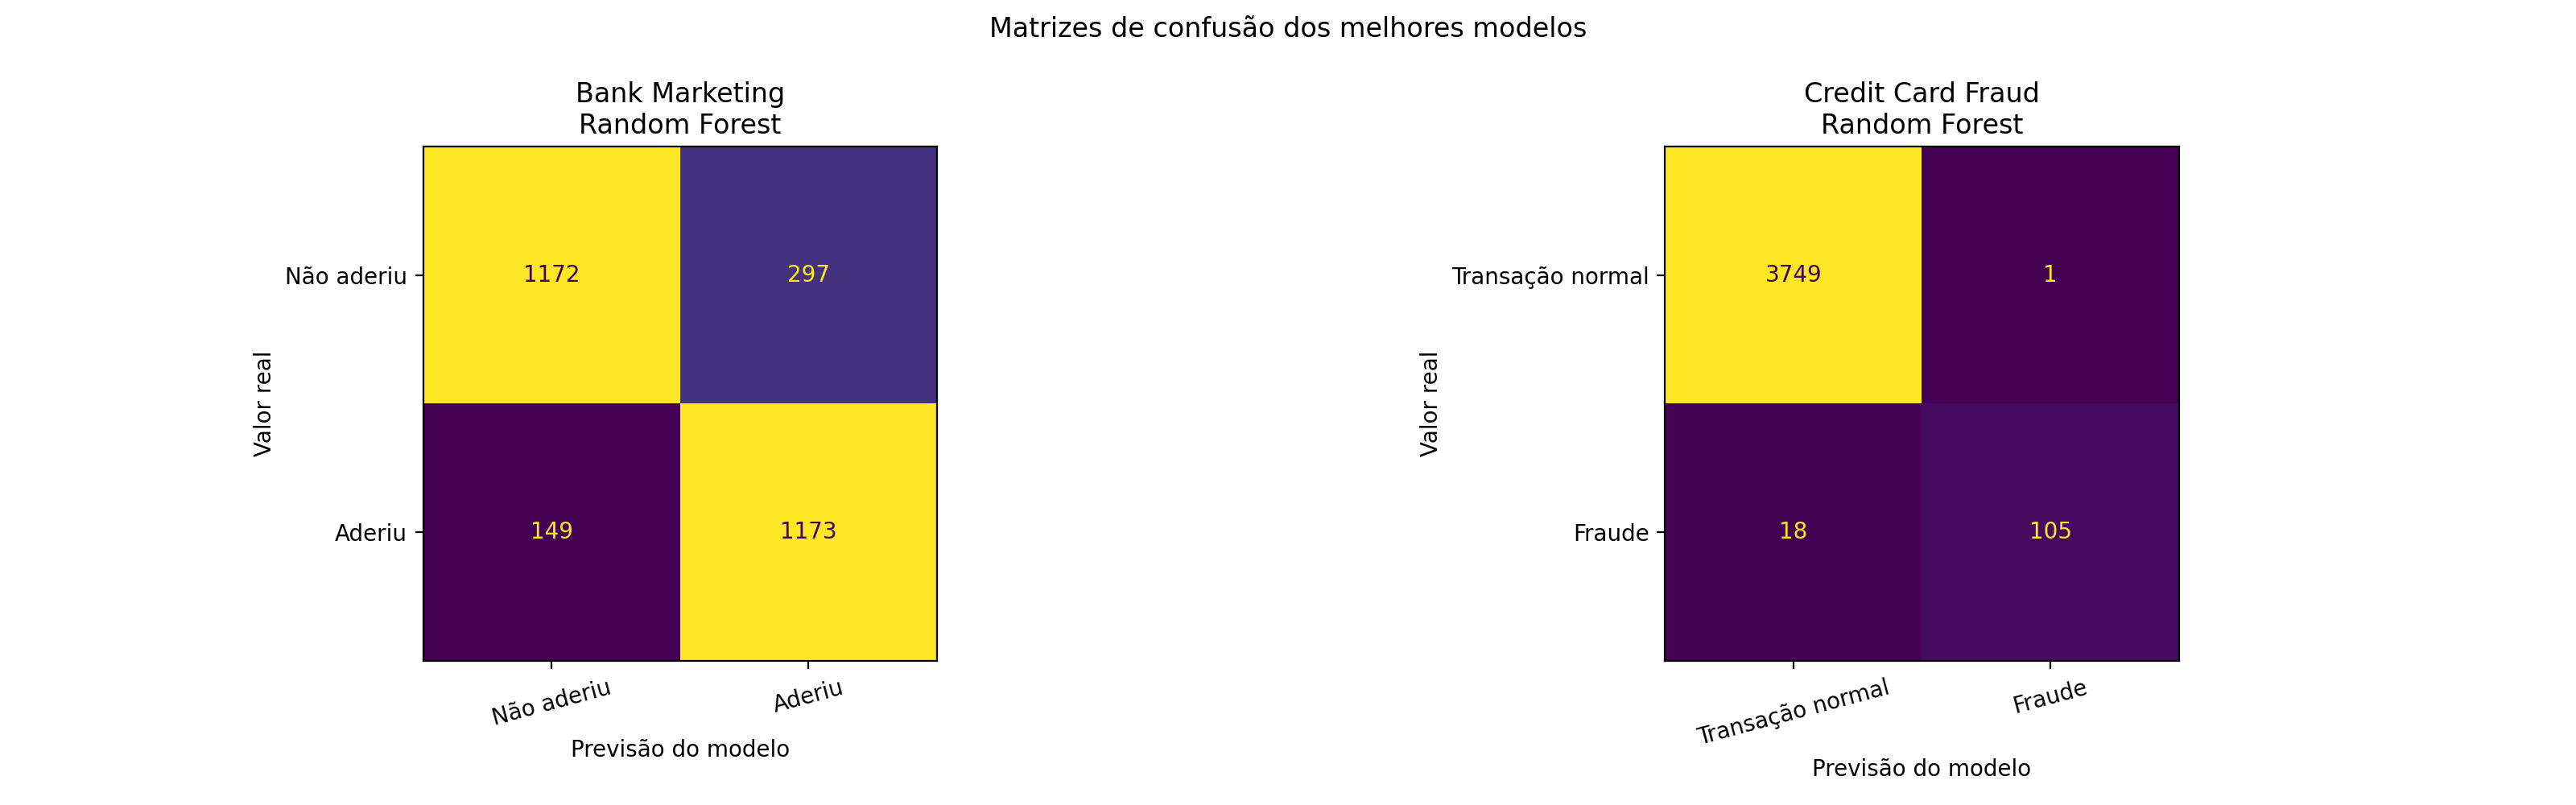
\includegraphics[width=0.95\linewidth]{../figures/confusion_matrix_best_model.png}
\caption{Matrizes de confusão do melhor modelo em cada dataset: Random Forest no Bank Marketing e Random Forest no Credit Card Fraud.}
\label{fig:confusion}
\end{figure}

No contexto da fraude, os falsos negativos são particularmente importantes, pois representam fraudes que passaram despercebidas. Contudo, os falsos positivos também têm custo operacional, porque podem bloquear operações legítimas ou gerar alertas desnecessários. Por isso, o melhor modelo deve procurar um equilíbrio entre reduzir fraudes não detetadas e evitar falsos alarmes.

\subsection{Comparação entre modelos}
A Figura~\ref{fig:f1} compara o F1-score dos três modelos nos dois datasets. O ranking global é consistente: o Random Forest é o melhor modelo em ambos os cenários. No Bank Marketing, a vantagem é moderada; no Credit Card Fraud, a diferença para Decision Tree e Regressão Logística é mais evidente.

\begin{figure}[H]
\centering
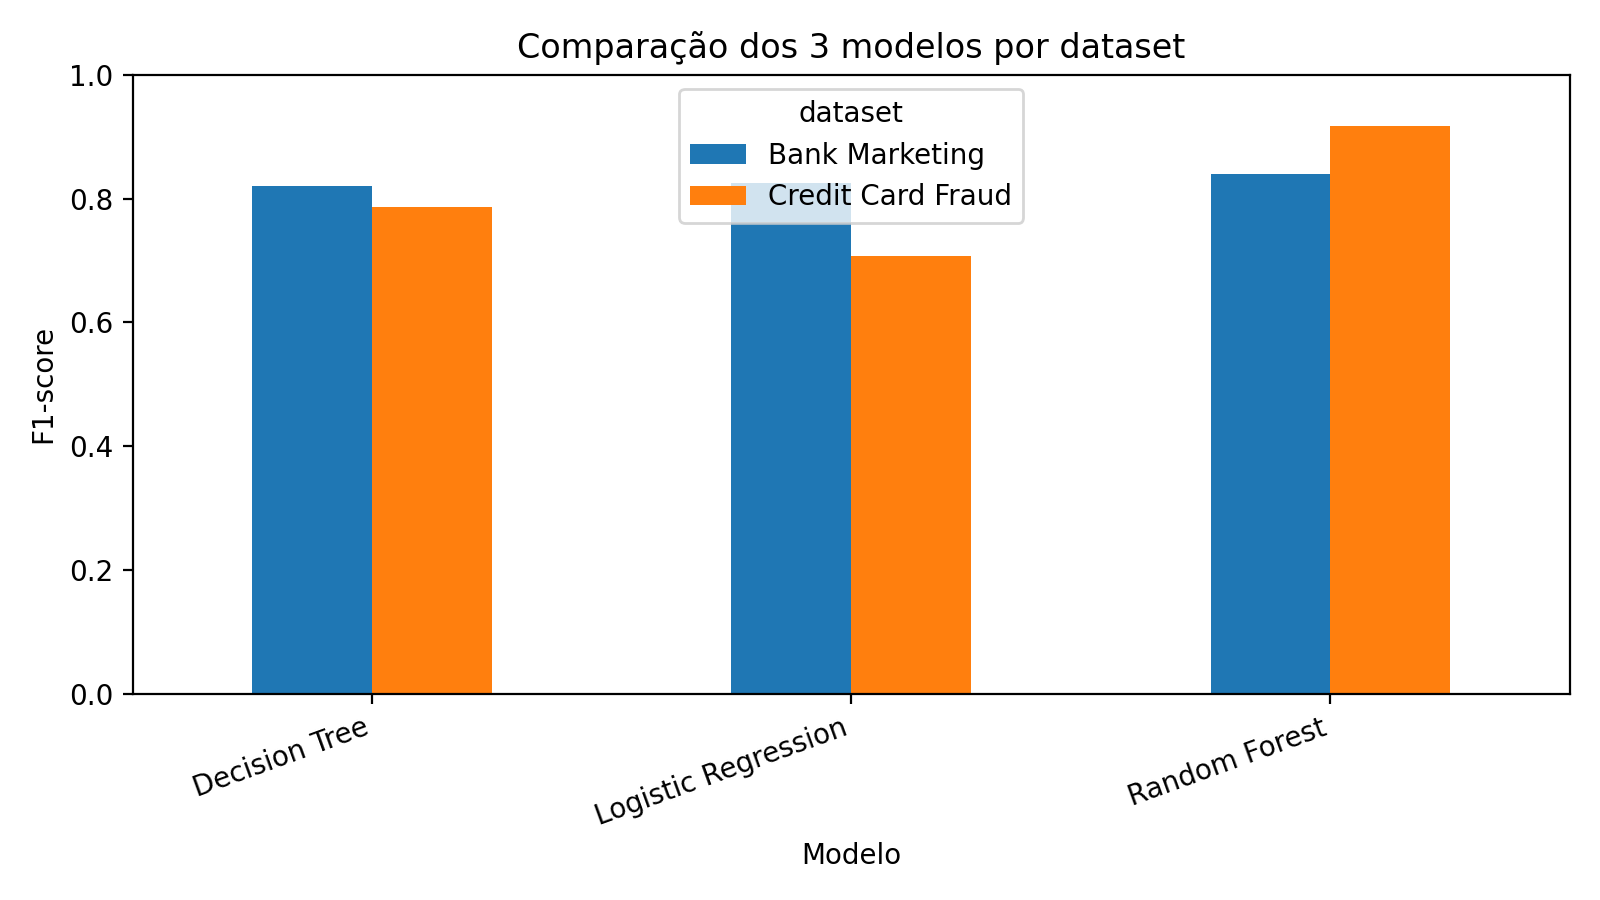
\includegraphics[width=0.95\linewidth]{../figures/model_f1_comparison.png}
\caption{Comparação do F1-score por modelo e por dataset.}
\label{fig:f1}
\end{figure}

A Decision Tree apresenta desempenho aceitável e interpretabilidade superior, mas perde para o Random Forest, sobretudo porque uma árvore isolada é mais sensível ao ruído. A Regressão Logística é competitiva no Bank Marketing e mostra recall elevado no Credit Card Fraud, mas a baixa precision no dataset de fraude indica que o modelo sinaliza muitos casos legítimos como suspeitos.

\subsection{Curvas ROC}
As curvas ROC fornecem uma análise complementar ao valor pontual das métricas. A curva ROC mostra a relação entre a taxa de verdadeiros positivos e a taxa de falsos positivos. Quanto mais próxima estiver do canto superior esquerdo, melhor é a capacidade do modelo distinguir as duas classes.

\begin{figure}[H]
\centering
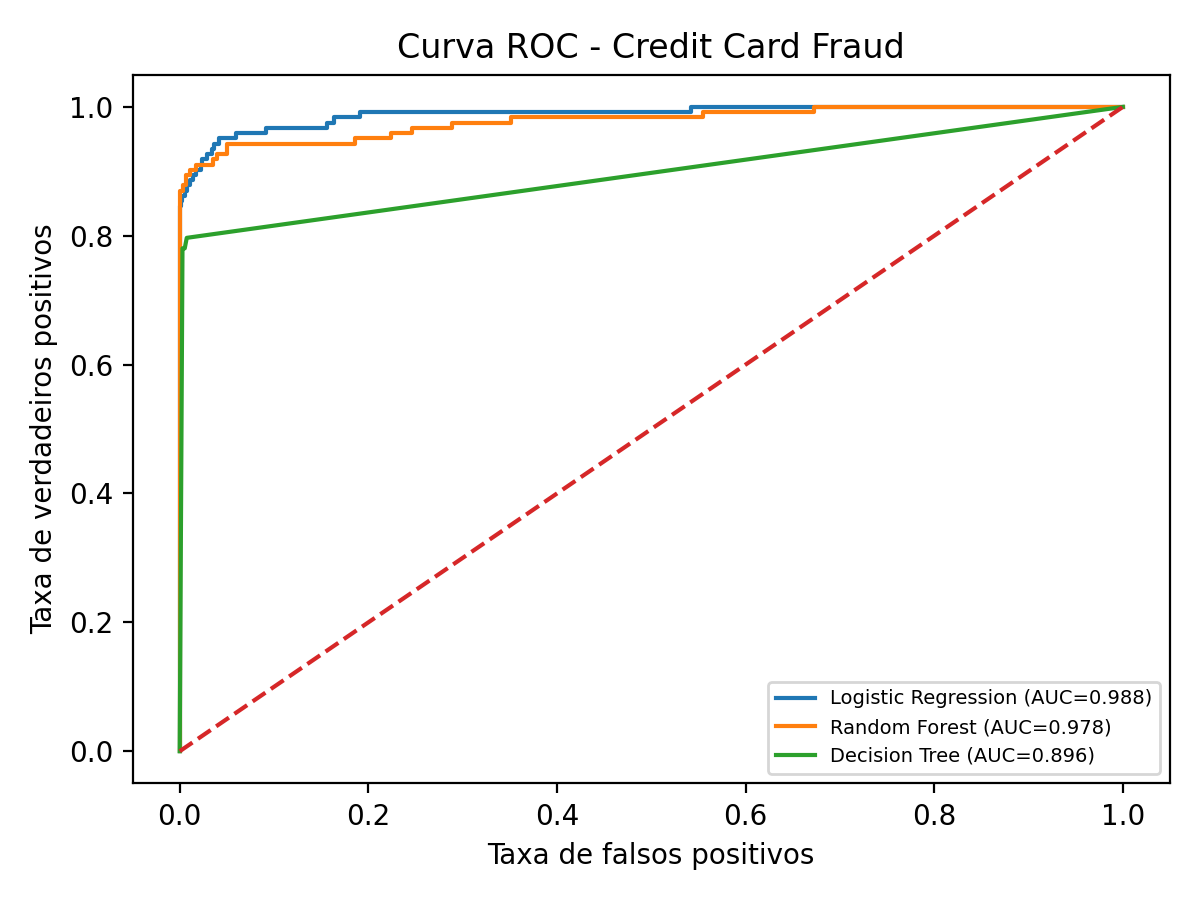
\includegraphics[width=0.95\linewidth]{../figures/roc_curve_models.png}
\caption{Curvas ROC dos modelos avaliados.}
\label{fig:roc}
\end{figure}

Os valores de ROC-AUC são elevados para os modelos principais, sobretudo no Credit Card Fraud. No entanto, em problemas muito desbalanceados, a ROC-AUC pode parecer muito positiva mesmo quando a precision não é suficiente. Por isso, a curva Precision-Recall é também analisada.

\subsection{Curvas Precision-Recall}
A curva Precision-Recall é particularmente relevante quando existe desequilíbrio entre classes, como acontece no Credit Card Fraud. Esta curva foca a qualidade da deteção da classe positiva, avaliando o compromisso entre encontrar muitos positivos e manter poucos falsos positivos.

\begin{figure}[H]
\centering
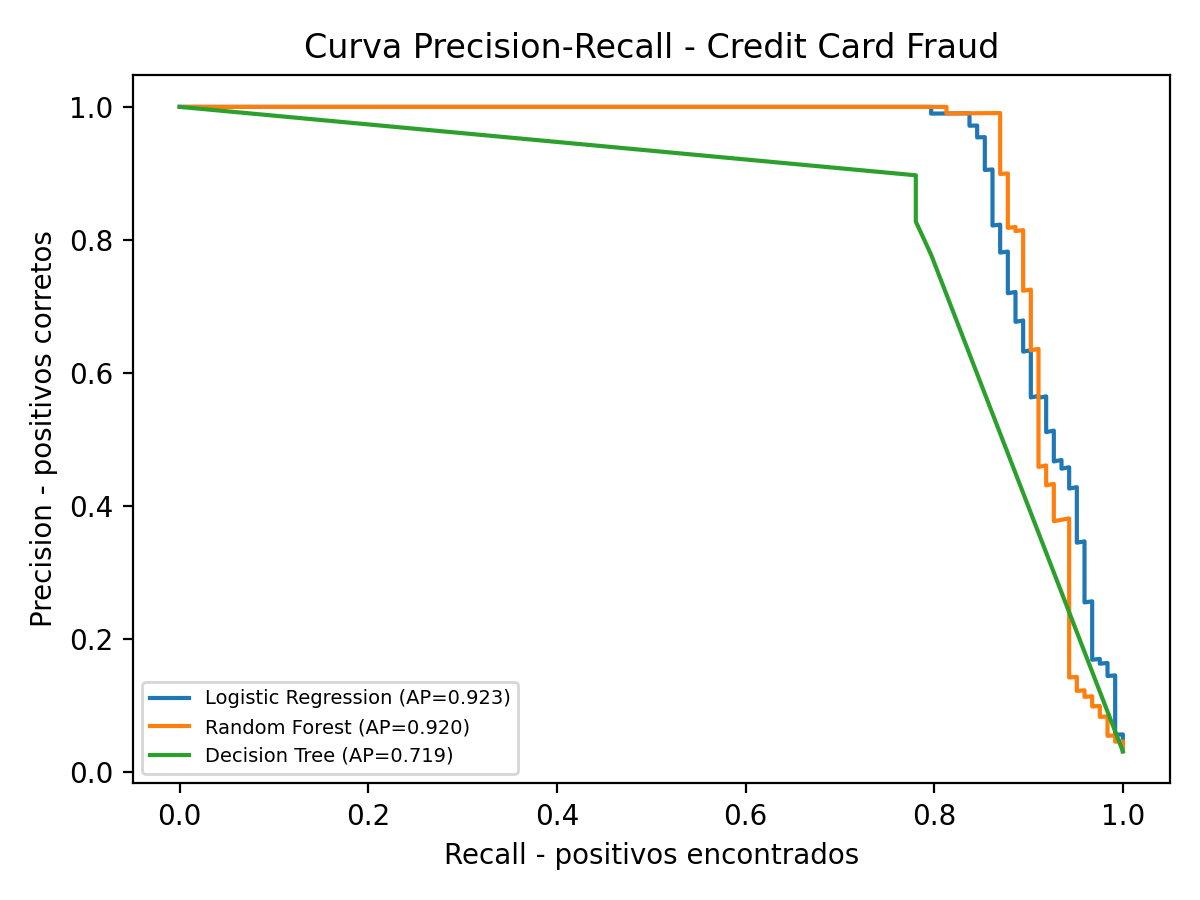
\includegraphics[width=0.95\linewidth]{../figures/precision_recall_curve_models.png}
\caption{Curvas Precision-Recall dos modelos avaliados.}
\label{fig:pr}
\end{figure}

No Credit Card Fraud, a Average Precision da Regressão Logística (0,9233) é muito próxima da do Random Forest (0,9199), mas o F1-score final é bastante inferior devido ao limiar de classificação utilizado. Isto indica que o modelo linear pode ordenar bem os exemplos por risco, mas a decisão binária final produz mais falsos positivos. O Random Forest apresenta um equilíbrio mais favorável no ponto de decisão usado.

\begin{table}[H]
\centering
\caption{Melhor modelo em cada dataset, de acordo com o F1-score.}
\label{tab:bestmodels}
\begin{tabular}{lcc}
\toprule
Dataset & Melhor modelo & F1-score \\
\midrule
Bank Marketing & Random Forest & 0,8403 \\
Credit Card Fraud & Random Forest & 0,9170 \\
\bottomrule
\end{tabular}
\end{table}

A Tabela~\ref{tab:bestmodels} resume o resultado principal do trabalho: nos dois datasets, o Random Forest foi o modelo que apresentou melhor equilíbrio entre encontrar os casos positivos e evitar falsos alarmes.

\subsection{Comparação entre datasets}
A comparação entre datasets mostra que o comportamento dos modelos depende fortemente da distribuição dos casos e da natureza dos atributos. No Bank Marketing, os três modelos obtêm resultados próximos, porque o dataset é mais equilibrado e a classe positiva representa quase metade dos exemplos. No Credit Card Fraud, o forte desequilíbrio torna a avaliação mais exigente: pequenas variações no número de falsos positivos ou falsos negativos têm impacto significativo na precision, no recall e no F1-score.

Do ponto de vista de cibersegurança, os falsos negativos são particularmente importantes, pois correspondem a fraudes não detetadas. Contudo, os falsos positivos também têm custo operacional. Assim, o melhor modelo não é necessariamente o que maximiza apenas o recall, mas sim o que oferece melhor compromisso entre recall e precision. Neste critério, o Random Forest é a opção mais consistente nos dois datasets.

\subsection{Discussão geral}
Os resultados confirmam que modelos supervisionados clássicos continuam a ser úteis em problemas financeiros de classificação binária. A Regressão Logística é rápida, simples e adequada como modelo de referência. A Decision Tree oferece interpretabilidade, mas menor estabilidade. O Random Forest apresenta o melhor desempenho global, especialmente quando existem relações não lineares ou interações entre atributos.

A principal limitação do trabalho é o uso de apenas dois datasets e três modelos, por opção metodológica e para manter a comparação controlada. Também não foi realizada uma otimização extensa de hiperparâmetros, de modo a preservar a simplicidade e a reprodutibilidade. Em trabalho futuro, seria relevante testar técnicas específicas para dados desbalanceados, como ajuste de limiar, reamostragem, SMOTE ou modelos com pesos de classe, além de avaliar o impacto operacional dos falsos positivos e falsos negativos.

\section{Conclusão}
Este trabalho apresentou uma comparação experimental entre Regressão Logística, Decision Tree e Random Forest em dois datasets financeiros: Bank Marketing e Credit Card Fraud. A metodologia foi construída como uma fluxo de processamento simples e reprodutível, com análise exploratória inicial, pré-processamento adequado, divisão treino/teste estratificada e avaliação com métricas apropriadas para classificação binária.

Os resultados mostram que o Random Forest foi o modelo mais eficaz em F1-score nos dois datasets, alcançando 0,8403 no Bank Marketing e 0,9170 no Credit Card Fraud. No dataset de fraude, a Regressão Logística obteve recall elevado, mas com baixa precision, mostrando que a deteção de fraude exige equilíbrio entre capturar eventos suspeitos e evitar falsos alarmes. A Decision Tree apresentou resultados razoáveis, mas inferiores ao ensemble de árvores.

Conclui-se que a utilização de aprendizagem supervisionada é adequada para apoiar a deteção de risco e fraude financeira. Entre os modelos avaliados, o Random Forest oferece a solução mais consistente, embora a escolha final em ambiente real deva considerar não apenas métricas estatísticas, mas também custo operacional, interpretabilidade, tempo de execução e tolerância a falsos positivos e falsos negativos.

\begin{thebibliography}{00}
\bibitem{dalpozzolo2014credit} A. Dal Pozzolo, O. Caelen, Y.-A. Le Borgne, S. Waterschoot, and G. Bontempi, ``Learned lessons in credit card fraud detection from a practitioner perspective,'' 2014.
\bibitem{moro2014data} S. Moro, P. Cortez, and P. Rita, ``A data-driven approach to predict the success of bank telemarketing,'' \emph{Decision Support Systems}, vol. 62, pp. 22--31, 2014.
\bibitem{breiman2001random} L. Breiman, ``Random forests,'' \emph{Machine Learning}, vol. 45, pp. 5--32, 2001.
\bibitem{pedregosa2011scikit} F. Pedregosa et al., ``Scikit-learn: Machine Learning in Python,'' \emph{Journal of Machine Learning Research}, vol. 12, pp. 2825--2830, 2011.
\bibitem{bhattacharyya2011data} S. Bhattacharyya, S. Jha, K. Tharakunnel, and J. C. Westland, ``Data mining for credit card fraud: A comparative study,'' \emph{Decision Support Systems}, vol. 50, no. 3, pp. 602--613, 2011.
\bibitem{chawla2002smote} N. V. Chawla, K. W. Bowyer, L. O. Hall, and W. P. Kegelmeyer, ``SMOTE: Synthetic minority over-sampling technique,'' \emph{Journal of Artificial Intelligence Research}, vol. 16, pp. 321--357, 2002.
\end{thebibliography}

\end{document}
